This spring-mass-pendulum-based example is presented to introduce \bioptim 's ability to use external forces.
The goal was to hold the position of a $\SI{1}{\kilo\gram}$ mass hanging on a linear spring attached to the ground.
A $\SI{0.2}{\meter}$-long pendulum weighting $\SI{10}{\kilo\gram}$ was attached to the mass and free to rotate in one dimension (Fig.~\ref{fig:Mass_Pendulum_Model}).
In addition to the spring force, the mass was actuated by a vertical external force (e.g., something pulling on it) while the pendulum rotation was passive.
The system therefore comprised two DoFs, the mass position ($q_m$) and the pendulum angle ($q_p$) and one control input, the vertical external force pulling on the mass ($\tau$). 
The spring force $\mathcal{F}_s$ was:
\[
\begin{aligned}
\tau_s = -k*q_m,
\end{aligned}
\addtag
\label{eq:f_ext}
\]
with $k$ the spring stiffness constant.\\
The OCP was composed of two phases each lasting for $\SI{5}{\second}$, with 50 shooting nodes.
In the first phase, no objective function was minimized and $\tau$ was constrained to be $0$, letting the mass oscillating freely. 
Then, in the second phase, a cost function (Eq.~\ref{eq:ocp_Pendulum}) was minimized, to enforce a reference position $q_m^*$ of the mass.
This objective function, exclusively composed of Lagrange terms, was formulated as follows:
\[
\mathcal{J} = \int_{T/2}^T \underbrace{ (q_m - q_m^*)^2}_{\mathtt{TRACK\_STATE}}  +~\omega_1 \underbrace{\tau^2~dt}_{\mathtt{MIN\_ TORQUE}}~dt,
\addtag
\label{eq:ocp_Pendulum}
\]

\noindent with $q_m^* = \SI{-0.5}{\meter}$ and $\omega_1 = 10^{-6}$ and T is the duration of the movement.
The first term of the objective function (Eq.~\ref{eq:ocp_Pendulum}) acts as a position controller for the mass.
The second was added for control regularization.

\begin{figure*}[t!]
\centering
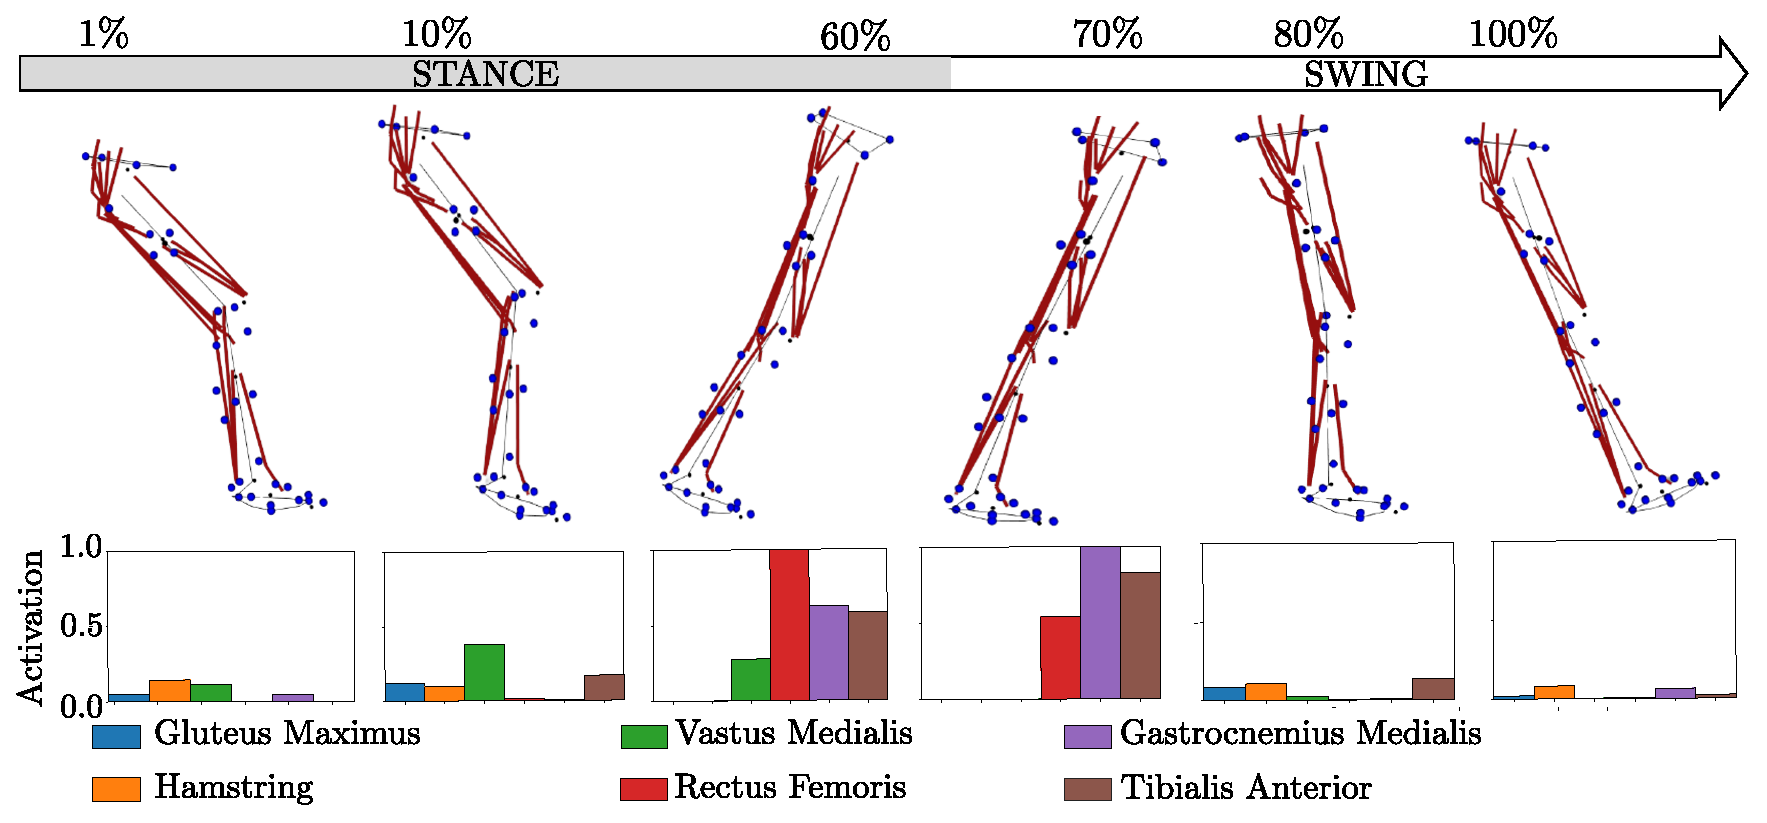
\includegraphics[width=\textwidth]{figures/multiphase_walking_cycle.eps}
\caption{Snapshots of a walking gait cycle driven by muscles activation with histogram of muscle activations below. The red lines represent muscles lines of action and the blue points depict the tracked markers. The activation of the Gluteus Maximus is the mean of its three parts and the Hamstring is the mean activation of the Semimembranous, Semitendinous and Biceps Femoris.}
\label{fig:snapshots_multiphase_walking_cycle}
\vspace*{-0.5cm}
\end{figure*}

During the first phase, the mass is passively oscillating around its stationary position due to the spring force (Fig.~\ref{fig:Mass_Pendulum_Fext_graphs}).
At the beginning of the second phase, when an additional external force acts on the mass, it stabilizes around the targeted position.
The standard deviation between the position and the targeted position is $\SI{0.04}{\m}$.
This example highlights the possibility of using optimal control to find activation patterns compensating for external passive forces (e.g., ortheses flexibility, contact surface deformation, interaction between two models, etc.).
\newpage